%!TEX ROOT = thesis.tex
\chapter{Introduction}
\section{Basic Introduction}
%In the Introduction section, you should describe the problem investigated. Try to summarize relevant research to provide context, key terms, and concept so the reader can understand the whole final year project. Go and read journal or conference papers and review relevant past research to 
%provide rational or justification for your work. Define clearly your final project objectives and briefly describe your research – design, 
%research, hypothesis, etc.
%Currently, the amount of vehicles on the road increases every year in Malaysia. It is because the local brand car is affordable by many low-income level households. The manufacturer also provided promotions to attract people to buy cars. As the result, the number of non-professional driver rapidly increased in Malaysia. Most of the drivers are unskilled and lack of awareness on the traffic safety and vehicle condition. The driver's personal factors have become the main reason of causing the traffic incidents.

According to the statistics on drivers in Malaysia taken from official portal of Road Transport Department Malaysia shown in Figure\ref{fig:driver}, the number of drivers increases every year in Malaysia. The drivers got the license through driving examinations, but it does not mean that the drivers have good driving behaviour.
 
\begin{figure}[hbt!]\centering
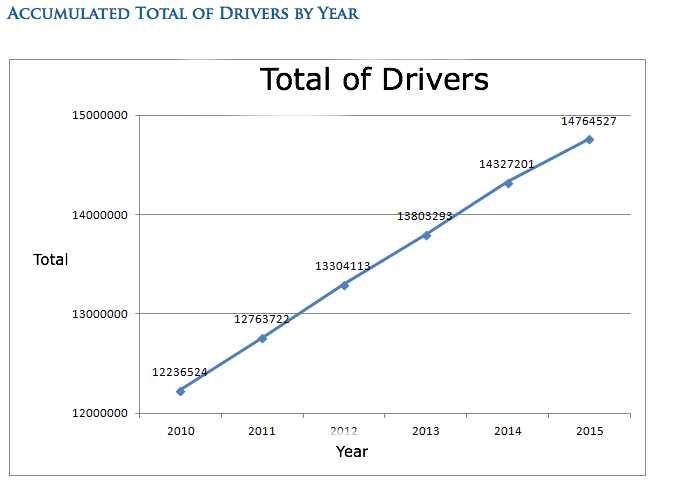
\includegraphics[width=.75\textwidth]{image/totaldriver}
\caption{Accumulated total of drivers by year (source from: http://www.jpj.gov.my/) }
\label{fig:driver}
\end{figure}

Based on the general road accident data in Malaysia taken from Malaysian Institute of Road Safety Research (MIROS) official website shown in Figure \ref{fig:accident}, Malaysia government put effort on reducing the amount of traffic incidents by introducing the new traffic laws and speed tracking system. However, the number of cases of road deaths does not drop significantly. It means that drivers' personal factors also related to the occurrence of traffic incident.

\begin{figure}[hbt!]\centering
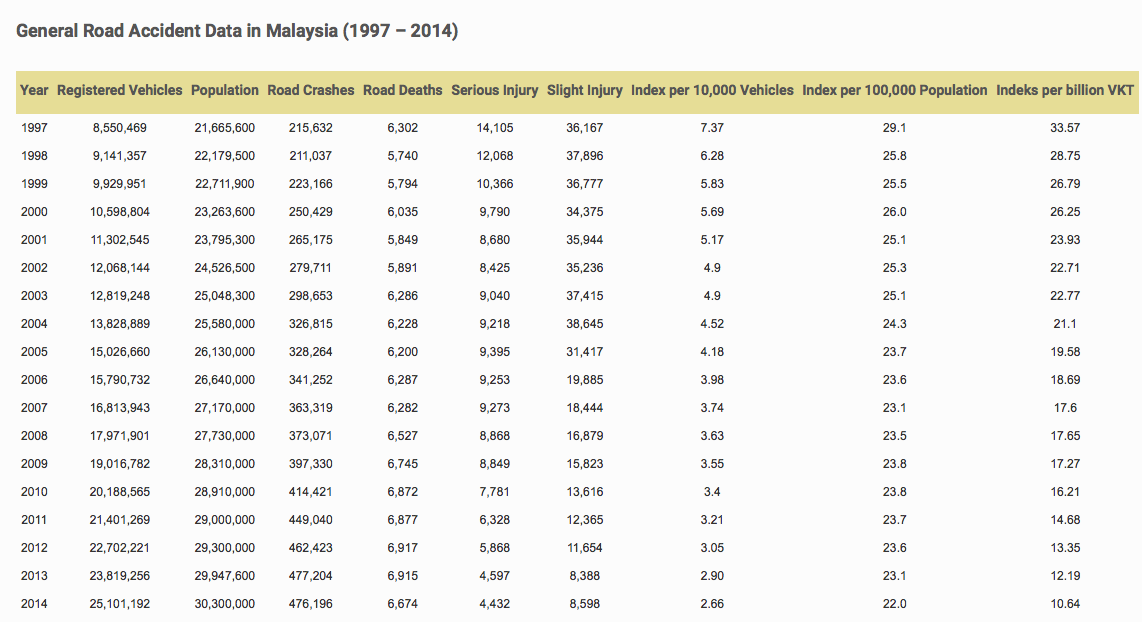
\includegraphics[width=.75\textwidth]{image/accident}
\caption{General Road Accident Data in Malaysia (1997 - 2014) (source from: https://www.miros.gov.my/)}
\label{fig:accident}
\end{figure}

The driver characteristics and the occurrence of traffic incident is interrelated. To further reduce the number of accidents, the safety equipment of the vehicle needs to be improved as well as the road regulations, but also pay attention to driver behaviour. However, the behaviour of the driver is hard to be identified. The driver behaviour is affected by environment, vehicle condition and the mental or physical state.\cite{miyaji:danno:oguri:2008} One of the ways to identify driver behaviour is using the vehicle telemetric data.

\section{Research Motivation}
This project might help insurance company to de-tariff the Motor Insurance in Malaysia. However, the insurance companies cannot obtain the vehicle telemetric data from customers directly. They cannot force their customers to drive without knowing that they are monitoring the customer's vehicle telemetric data.

Currently, new high end cars do send driving data back to the manufacturers. Consumer group Federation Internationale de I'Automobile (FIA) exposed Bayerische Motoren Werke AG (BMW) received data from their manufactured cars. The data actually can analyse driver driving behaviour.\cite{catherine:2015} So, the model built in this project can possibly be used when these insurance companies want to classify drivers. However, the insurance companies may classify the drivers with lesser data.

\section{Project Objective}
\begin{enumerate}
\item To identify the features that contributes to the accuracy of the classification of the driver behaviour analysis from the vehicle telemetric data.
\item To classify each vehicle telemetric records.
\item To profile the drivers based on the labelled vehicle telemetric data.
\end{enumerate}

\section{Project Scope}
This project focuses on driving behaviour analysis based on vehicle telemetric data and K-Means algorithm. Actual vehicle telemetric data are captured by sensor. The vehicle telemetric data will be collected and preprocessed before analysing. This project requires a vehicle that supports the On Board Diagnostic (OBD-II) device. Each driver is required to drive the vehicle for at least 8 minutes to collect data. The data will be recorded every second. For each driver, there are at least 480 records in the dataset. K-Means algorithm is implemented in this project to cluster the vehicle operation records. Each record will be labelled as good, medium or bad condition. Based on the labelled records, the drivers will be categorized to three classes. The classes are low risk, medium risk and high risk. 

\section{Project Plan}
Proper time and resource management is important to complete this project. Table \ref{tbl:gantt1} shows a brief description of the project timeline.

\begin{table}[h!]
\begin{tabular}{|l|c|c|c|c|c|c|c|c|c|c|c|}
\hline
Task \textbackslash Week & 2 & 3 & 4 & 5 & 6 & 7 & 8 & 9 & 10 & 11 & 12 \\

\hline
Data Acquisition &  \cellcolor[HTML]{000000} & \cellcolor[HTML]{000000} & \cellcolor[HTML]{000000} & \cellcolor[HTML]{000000} & \cellcolor[HTML]{000000} & & & & & & \\

\hline
Literature Review & & \cellcolor[HTML]{000000} & \cellcolor[HTML]{000000} & \cellcolor[HTML]{000000} & \cellcolor[HTML]{000000} & & & & & & \\

\hline
Data Analysis using KNIME & & & & & & \cellcolor[HTML]{000000} & \cellcolor[HTML]{000000} & \cellcolor[HTML]{000000} & & & \\

\hline
Driver Driving Behaviour Profiling & & & & & & & & \cellcolor[HTML]{000000} & \cellcolor[HTML]{000000} &  & \\

\hline
Analysing Experimental Result & & & & & & & & & \cellcolor[HTML]{000000} & \cellcolor[HTML]{000000} & \\

\hline
Documentation and Report & & & & & & & & & \cellcolor[HTML]{000000} & \cellcolor[HTML]{000000} & \cellcolor[HTML]{000000} \\

\hline
Report Submission & & & & & & & & & & & \cellcolor[HTML]{000000}\\

\hline
\end{tabular}
\label{tbl:gantt1}
\caption{Project timeline of Final Year Project I for Trimester 1 2016/2017}
\end{table}